\chapter{Anforderungen}
\label{chap:Anforderungen}
In diesem Kapitel werden die Anforderungen an den Elektrolysegleichrichter von beiden Seiten beschrieben. Auf der einen Seite fordert der Netzbetreiber die Einhaltung der Richtlinien für den Netzanschluss, welche vom \gls{VDE} definiert werden. Dies wird meist als Einhaltung der anerkannten Regeln der Technik zusammengefasst. Die andere Seite wird durch den Hersteller des Elektrolyseur-Stacks definiert, für den es nach heutigem Stand keine Normen für die elektrischen Anforderungen gibt. 
\section {Stromnetz} \label{sec:AnfStromnetz}
In Deutschland sind die Anforderungen an den Netzanschluss von Anlagen durch den \gls{VDE} festgelegt. Je nach Anschlussleistung, Standort und Betriebsverhalten wird eine unterschiedliche Netzspannungsklasse gewählt, die leicht abweichende Anschlussrichtlinien besitzt. Aufgrund der Skalierbarkeit zu höheren Leistungsklassen und den zu erwartenden steigenden Anforderungen wird die Hochspannungsklasse gewählt. Dies ist die VDE-AR-N 4120 \glqq Technische Regeln für den Anschluss von Kundenanlagen an das Hochspannungsnetz und deren Betrieb (TAR Hochspannung)\grqq \cite{VDEARN4120}.
Diese beinhaltet u.~a. die Anforderung an die Phasenverschiebung, bei Wirkleistungsbezug darf eine maximale Verschiebung von $cos(\phi)=0,95$ auftreten, was einem Winkel von ca. 18 Grad entspricht, vgl. Abbildung \ref{fig:tar4120pq}. Der Netzbetreiber kann jedoch mit dem Anlagenbetreiber gesonderte Vereinbarungen treffen, die es ermöglichen, Netzdienstleistungen anzubieten. Daraus ergibt sich die Anforderung an die Topologie, eine Phasenverschiebung von mindestens 18 Grad zu ermöglichen.\\
\begin{figure}
	\centering
	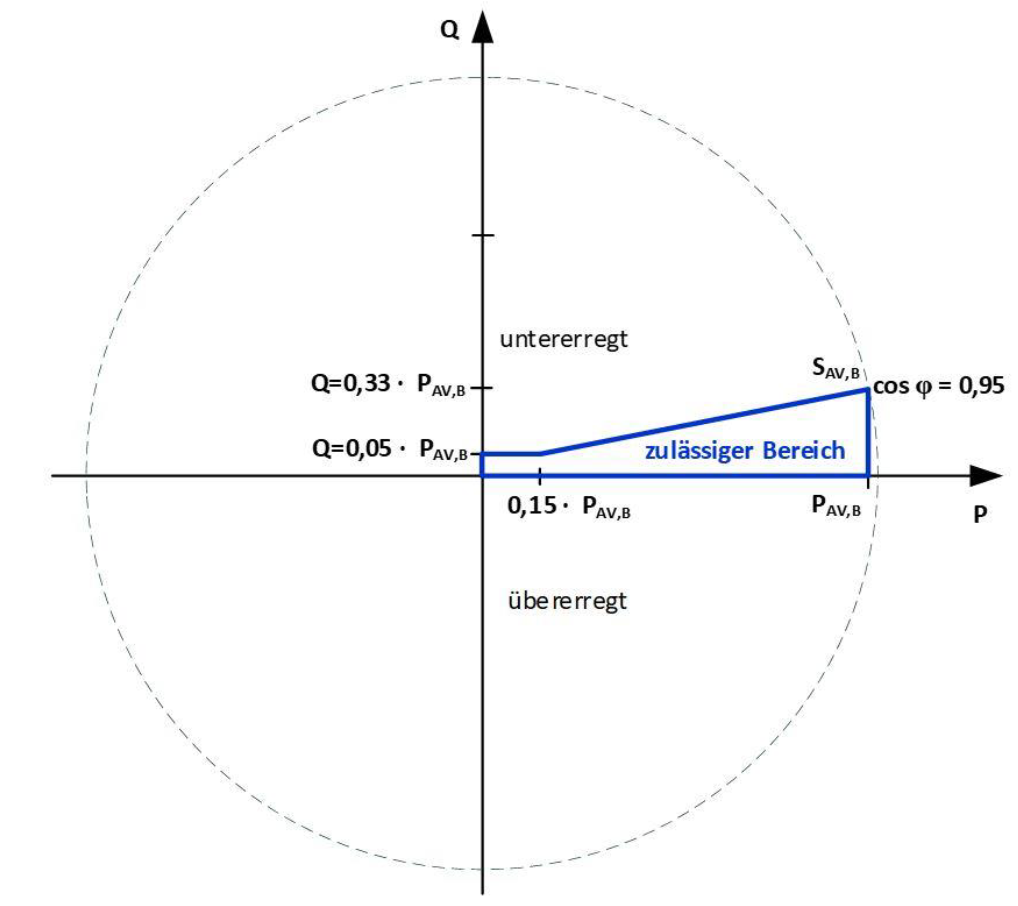
\includegraphics[width=0.6\linewidth]{content/Grafiken/TAR4120_PQ}
	\caption[Zulässiger Bereich des Verschiebungsfaktors cos $\phi$ bei Wirkleistungsbezug]{VDE TAR4120: Zulässiger Bereich des Verschiebungsfaktors \cite{VDEARN4120}}
	\label{fig:tar4120pq}
\end{figure}
Als quasistationärer Betrieb werden auch zeitlich begrenzte Frequenz- und Spannungsänderungen definiert, die auftreten können. Die Netzspannung darf im Bereich von +/- 15 Prozent schwanken, die Frequenz von 50 Hertz zwischen 47,5 und 51,5 vgl. Abb. \ref{fig:vde4120-Anforderungen} (a). Innerhalb dieses Bandes muss die Anlage im Regelbetrieb bleiben. Dies setzt einen Gradienten von <5 \% im Spannungsband und <0,5 \% pro Minute im Frequenzband voraus. \\
Im Fehlerfall durch Blitzeinschlag oder Kurzschluss muss die Anlage kurzzeitig deutlich größere Spannungsschwankungen ertragen. Diese Anforderung wird als \glsentrylong{FRT} (\gls{FRT}) bezeichnet und kann die Spannung für bis zu 100 Millisekunden um 25 Prozent erhöhen, siehe Abbildung \ref{fig:vde4120-Anforderungen} (b). Durch einen Kurzschluss kann die Spannung auf 15 Prozent der eigentlichen Netzspannung absinken. Dies stellt für Verbraucheranlagen eine große Herausforderung dar, da die zu betreibenden Systeme in der Regel eine Mindestspannung benötigen.

\begin{figure}
\centering
\subfloat[][]{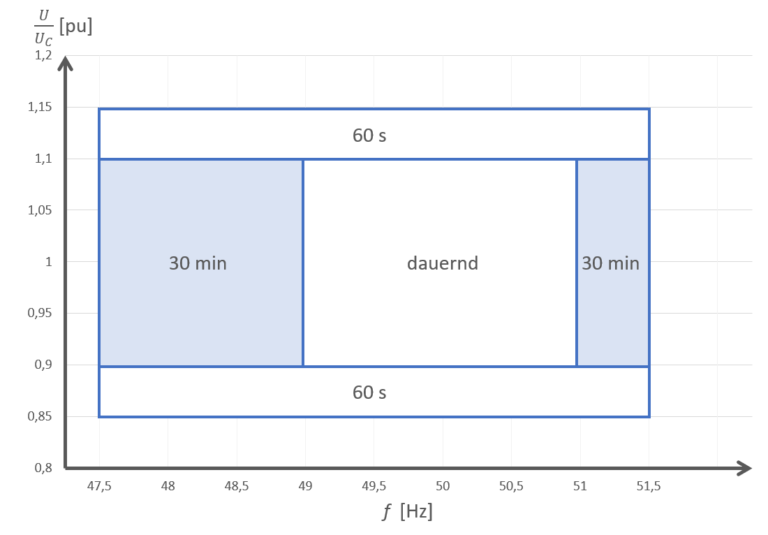
\includegraphics[width=0.9\linewidth]{content/Grafiken/VDE4120-quasistationarerbetrieb}}%
%\caption[Mindestanforderungen an den quasistationären Betrieb von Erzeugungsanlagen \cite{VDEARN4120]{Quasistationärer Betrieb}}
\qquad
\subfloat[][]{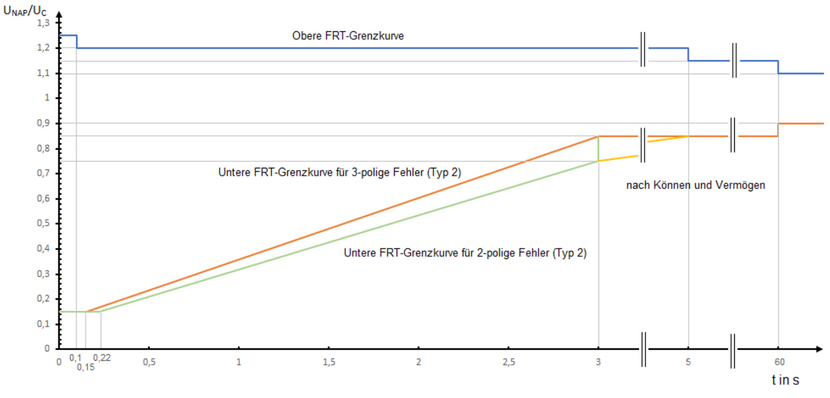
\includegraphics[width=0.9\linewidth]{content/Grafiken/Grenzkurve}}%
\caption{Mindestanforderungen an den quasistationären Betrieb (a) und \gls{FRT} (b) \cite{VDEARN4120}}
\label{fig:vde4120-Anforderungen}
\end{figure}




	\subsection{Systemdienstleistungen}
	Generell ist die Bundesnetzagentur für die Regulierung und Überwachung aller Dienstleistungen und Aktivitäten im deutschen Netz zuständig. Dazu gehört auch die Bereitstellung und Sicherstellung von Blindleistung, die effizient, transparent und diskriminierungsfrei am Markt zu beschaffen ist. Hierfür bieten sich in Zukunft große Verbrauchseinrichtungen wie Elektrolyseure neben Erzeugungsanlagen an und diese Dienstleistungen können die Wirtschaftlichkeit der Wasserstofferzeugung erhöhen.\\
	Die Systemdienstleistungen werden nach VDE-ARN 4141-1 in vier Kategorien unterteilt: Frequenz- und Spannungshaltung, Netzwiederaufbau und Betriebsführung. Die \gls{TAR} definiert diese und stellt Anforderungen an den Nachweis und die Ausschreibung von \gls{SDL}. Eine Übersicht über die technischen Mindestanforderungen an Erzeugungsanlagen in den verschiedenen Spannungsklassen zeigt Abb. \ref{fig:vde-fnn-tar}. Frequenzschwankungen stellen für stromrichterbasierte Elektrolyseanlagen kaum eine Herausforderung dar, diese können durch Regelvorgänge kompensiert und Netzstützung, wie bei \gls{RoCoF} erforderlich, bereitgestellt werden. Bei \gls{RoCoF} handelt es sich um schnelle Frequenzänderungen, wie sie bei einer Netztrennung oder -wiederverbindung auftreten. Primärregelleistung, statische Spannungshaltung und dynamische Netzstützung können ebenfalls durch Regelverhalten realisiert werden, sind jedoch begrenzt durch die Dynamik und den Leistungsbezug des Elektrolyseurs. Netzrückwirkungen sind ebenfalls zu berücksichtigen und können durch entsprechende Filter kompensiert werden. Die Schwarzstartfähigkeit ist als Verbraucheranlage nicht möglich und kann nur durch eine Leistungsbegrenzung während des Wiederaufbaus unterstützt werden.
	\begin{figure}
		\centering
		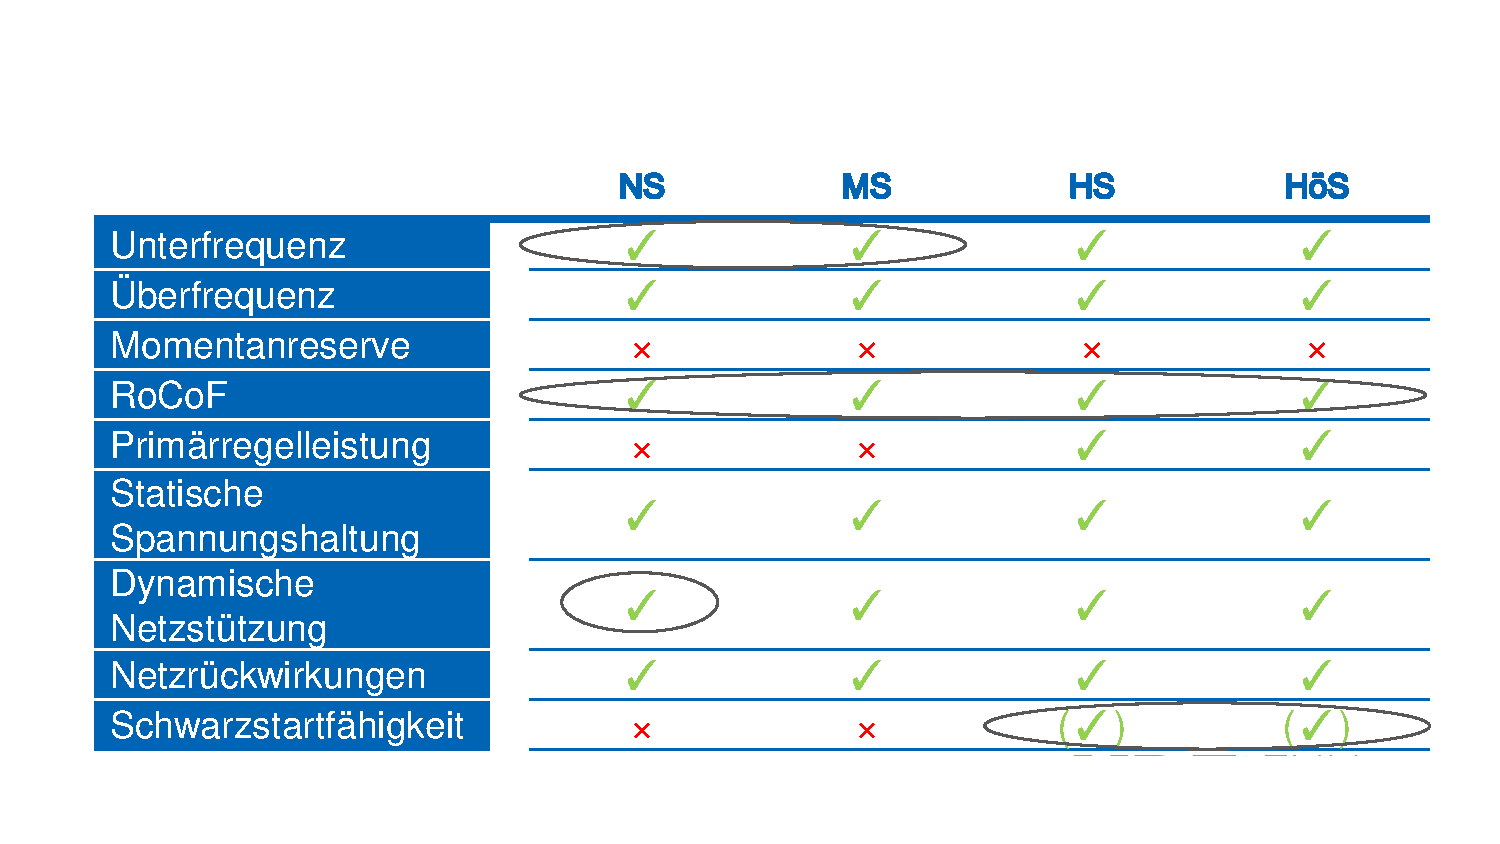
\includegraphics[width=0.9\linewidth]{content/Grafiken/VDE-FNN-TAR}
		\caption[Technische Mindestanforderungen an Erzeugungsanlagen Stand 2019]{Technischen Mindestanforderungen an Erzeugungsanlagen Stand 2019 \cite{VDEFNN2019SDL}}
		\label{fig:vde-fnn-tar}
	\end{figure}
	
	
	
	
	\subsection{Fault-Ride-Through (FRT)}
	Aufgrund von Netzfehlern oder Blitzeinschlägen kann es zu einer kurzzeitigen Erhöhung der Netzspannung kommen, die als Überspannung bezeichnet wird. Diese Spannungserhöhung kann zu Fehlfunktionen bis hin zur Zerstörung von Anlagenteilen führen. Um die Anlage innerhalb der Norm betreiben zu können, müssen Schutzmaßnahmen getroffen werden, die einen Ausfall der Anlage und den Schutz der nachgeschalteten Komponenten gewährleisten.
	Insbesondere bei Spannungseinbrüchen ist es wichtig, dass der Wirkleistungsbezug nach dem Fehler möglichst schnell wieder auf das Niveau vor dem Fehler zurückkehrt, falls dieser reduziert wurde. Dies wird von den vier in Deutschland zuständigen Übertragungsnetzbetreibern gefordert \cite{4UNB}.


\section{Elektrolyseur}
Für die Elektrolyse wird eine Gleichspannung benötigt, die aufgrund von Alterungsprozessen in der Zellmembran mit der Zeit ansteigt \cite{HydrogenElectronicTopologies}. Außerdem wird zu Beginn der Elektrolyse eine niedrige Spannung benötigt, um den Prozess zu starten. Daher ist ein Bereich von 0 bis zu einigen 100 Volt erforderlich. Um die gewünschte Leistung umsetzen zu können, ist es für die Wirtschaftlichkeit relevant, den Strom so weit wie möglich zu reduzieren, was eine höhere Spannung zur Folge hat. Dies wird durch den modularen Zellaufbau unterstützt, der eine flexible Systemspannung ermöglicht. \\
Um den Wirkungsgrad und die Lebensdauer des Elektrolyseurs nicht zu verringern, wird ein maximaler Stromrippel vorgegeben. Dieser liegt für Anlagen bis 3 \si{\mega \watt} zwischen 5 und 10 \%, für größere Leistungen und zukünftige Anwendungen soll er unter 3 \% liegen \cite{HydrogenRectifier}.


\section{Zusammenfassung}
Die Anforderungen an den Gleichrichter sind in Tabelle \ref{tab:AnfZsm} zusammengefasst, für die Umsetzung sind die Zukünftigen Anforderungen relevant. \\
\begin{table}
	\centering
\caption{Anforderungen an den Gleichrichter Aktuell und in Zukunft}
\label{tab:AnfZsm}
\begin{tabular}{c|c|c}
	& Aktuell & Zukünftig \\
	\hline
	Leistungsfaktor stationär & >0.95 & >0.99 \\
	\hline
	Netzspannungsschwankung & 15 \% & 15 \% \\
	\hline
	Leistungsfaktor als Systemdienstleistung & keine Angabe & +/- 30° \\
	\hline
	Ausgangsstromrippel & <5 \% & <5 \% \\
	\hline
	Ausgangsspannung & 0..1000 V & 0..1500 V \\

\end{tabular}
\end{table}

%\section{Bewertungskriterien}
%Die Kriterien für die endgültige Auswahl der Topologie setzen sich aus der Erfüllung der Anforderungen und der Bewertung der Hardware zusammen. Die grundsätzlichen Anforderungen von Seiten des Stromnetzes und des Elektrolyseurs wurden bereits in der Vorauswahl berücksichtigt und können nun im Detail anhand von \gls{THD} und Rippelgrößen betrachtet werden. Die Quantifizierung der Hardware erfolgt zum einen über die Verlustleistung in den Halbleitern, die indirekt auch den Kühlungsaufwand abbildet, zum anderen über die Größe und den Aufwand der Komponenten.  